\documentclass[aspectratio=169,11pt]{beamer}

\usepackage[spanish,es-noshorthands]{babel}
\usepackage[T1]{fontenc}
\usepackage[utf8]{inputenc}
\usepackage{lmodern}
\usepackage{amsmath}
\usepackage{booktabs}
\usepackage{array}
\usepackage{tabularx}
\usepackage{graphicx}
\usepackage{xcolor}
\usepackage{ragged2e}

\definecolor{insblue}{RGB}{12,52,112}
\definecolor{insgold}{RGB}{198,150,33}
\definecolor{inslight}{RGB}{240,244,250}
\definecolor{insgreen}{RGB}{33,120,79}
\definecolor{insred}{RGB}{165,52,52}
\definecolor{insgray}{RGB}{90,98,110}
\definecolor{inssoft}{RGB}{248,250,253}

\usetheme{Madrid}
\usecolortheme{default}
\setbeamertemplate{navigation symbols}{}
\setbeamertemplate{blocks}[rounded][shadow=false]
\setbeamerfont{title}{series=\bfseries,size=\LARGE}
\setbeamerfont{subtitle}{series=\mdseries,size=\large}
\setbeamerfont{frametitle}{series=\bfseries,size=\Large}
\setbeamerfont{block title}{series=\bfseries}

\setbeamercolor{palette primary}{bg=insblue,fg=white}
\setbeamercolor{palette secondary}{bg=insblue,fg=white}
\setbeamercolor{palette tertiary}{bg=insblue,fg=white}
\setbeamercolor{structure}{fg=insblue}
\setbeamercolor{frametitle}{bg=insblue,fg=white}
\setbeamercolor{title}{fg=insblue}
\setbeamercolor{normal text}{fg=black,bg=white}
\setbeamercolor{background canvas}{bg=white}
\setbeamercolor{block title}{bg=insblue,fg=white}
\setbeamercolor{block body}{bg=inslight,fg=black}
\setbeamercolor{block title alerted}{bg=insred,fg=white}
\setbeamercolor{block body alerted}{bg=inssoft,fg=black}
\setbeamercolor{block title example}{bg=insgreen,fg=white}
\setbeamercolor{block body example}{bg=inssoft,fg=black}
\setbeamercolor{itemize item}{fg=insgold}
\setbeamercolor{itemize subitem}{fg=insblue}
\setbeamercolor{alerted text}{fg=insred}

\setbeamertemplate{frametitle}{
    \vskip0.05cm
    \begin{beamercolorbox}[wd=\paperwidth,ht=0.95cm,dp=0.25cm,leftskip=0.35cm,rightskip=0.35cm]{frametitle}
        \usebeamerfont{frametitle}\insertframetitle
    \end{beamercolorbox}
    {\color{insgold}\rule{\paperwidth}{1.2pt}}
}

\setbeamertemplate{footline}{
    \leavevmode
    \hbox{
    \begin{beamercolorbox}[wd=.68\paperwidth,ht=2.7ex,dp=1ex,leftskip=0.3cm]{author in head/foot}
        \color{insgray}\scriptsize César Zapata \hspace{0.4cm}|\hspace{0.4cm} Laboratorio ALAN TURING
    \end{beamercolorbox}
    \begin{beamercolorbox}[wd=.22\paperwidth,ht=2.7ex,dp=1ex,rightskip=0.3cm plus1fil]{date in head/foot}
        \color{insgray}\scriptsize \insertframenumber
    \end{beamercolorbox}}
}

\setbeamertemplate{title page}{
    \begin{columns}[c]
    \begin{column}{0.68\linewidth}
        \vspace{0.5cm}
        {\usebeamerfont{title}\color{insblue}\inserttitle\par}
        \vspace{0.25cm}
        {\usebeamerfont{subtitle}\color{insgold}\insertsubtitle\par}
        \vspace{0.5cm}
        {\usebeamerfont{author}\insertauthor\par}
        \vspace{0.15cm}
        {\usebeamerfont{institute}\insertinstitute\par}
        \vspace{0.15cm}
        {\usebeamerfont{date}\insertdate\par}
    \end{column}
    \begin{column}{0.28\linewidth}
        \centering
        
\includegraphics[width=0.96\linewidth]{../../../logo_ins.png}
    \end{column}
    \end{columns}
}

\title{Proyecto TD3 para Protesis Mioelectrica}
\subtitle{Desde la base conceptual hasta el agente residual final}
\author{César Zapata}
\institute{Laboratorio de Investigacion en Inteligencia y Vision Artificial ``ALAN TURING''}
\date{26 de marzo de 2026}

\begin{document}

\begin{frame}
\titlepage
\end{frame}

\begin{frame}{Problema y objetivo}
\begin{columns}[T]
\begin{column}{0.53\linewidth}
\begin{block}{Problema}
Queremos que una protesis siga una referencia de mano usando senales EMG y estado mecanico.
\end{block}
\begin{block}{Dificultad}
No basta con moverse: la politica debe evitar saturacion, esfuerzo excesivo y cambios bruscos.
\end{block}
\end{column}
\begin{column}{0.43\linewidth}
\begin{block}{Objetivo final}
\begin{itemize}
\item buen tracking
\item accion moderada
\item menos saturacion
\item resultado reproducible
\end{itemize}
\end{block}
\vspace{0.2cm}
\tiny Fuente conceptual: manuscrito base de Fuertes et al.; marco TD3 de Fujimoto et al. (2018).
\end{column}
\end{columns}
\end{frame}

\begin{frame}{Linea general del proyecto}
\centering
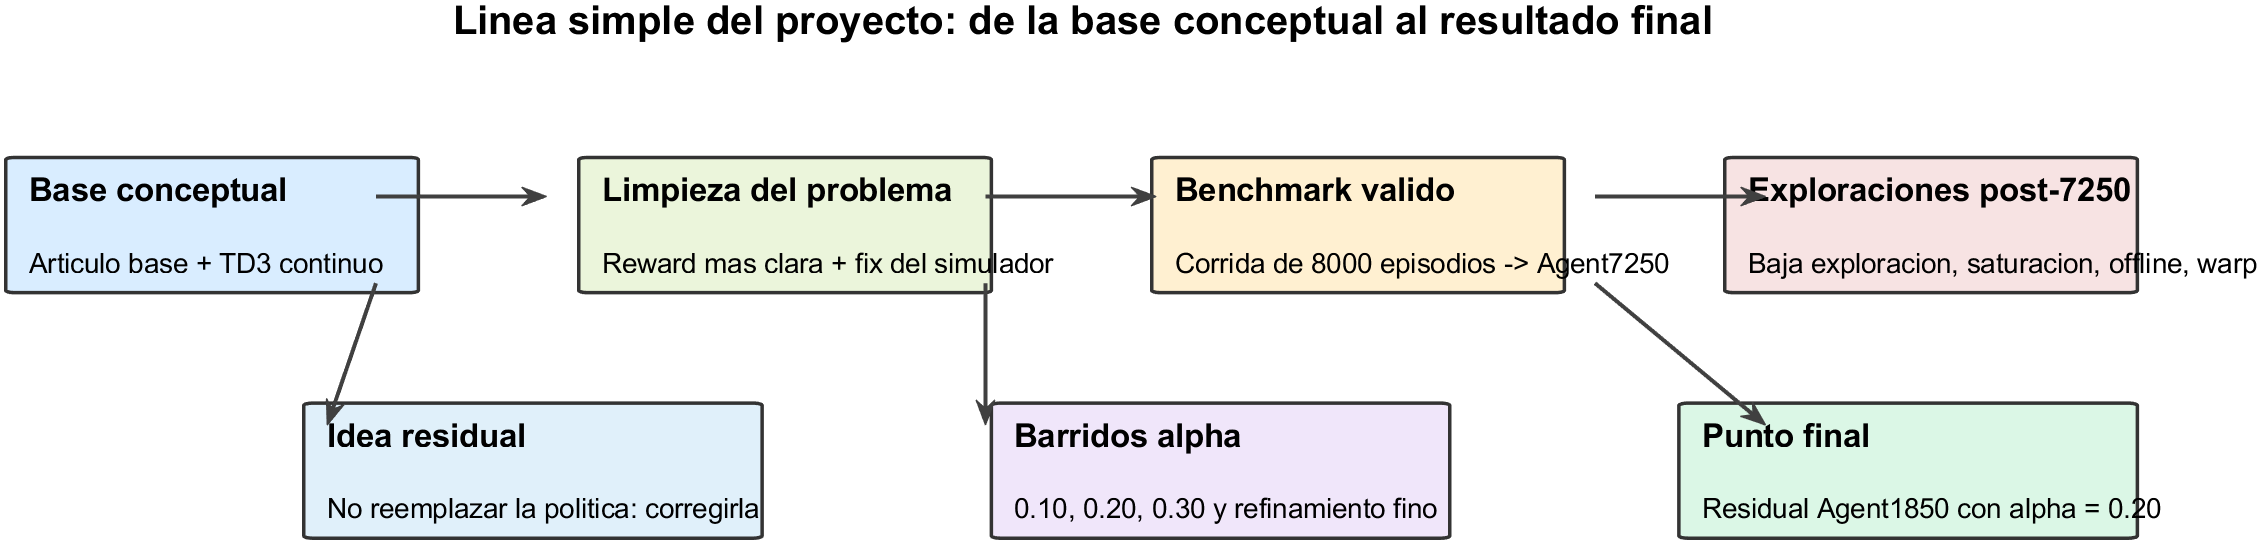
\includegraphics[width=0.97\linewidth]{figures/charla_linea_proyecto_20260326.png}
\vspace{0.2cm}

\small
La historia se divide en dos fases: primero obtener un benchmark valido; despues mejorarlo sin romper el tracking.
\end{frame}

\begin{frame}{Que hubo que arreglar antes de comparar agentes}
\begin{columns}[T]
\begin{column}{0.32\linewidth}
\begin{block}{Reward}
Se paso de una reward heredada poco interpretable a una reward centrada en tracking MSE.
\end{block}
\end{column}
\begin{column}{0.32\linewidth}
\begin{block}{Accion efectiva}
Se explicito el remapeo cuantizado a niveles PWM utiles para alinear politica y actuador.
\end{block}
\end{column}
\begin{column}{0.32\linewidth}
\begin{alertblock}{Simulador}
Se detecto un bug importante. Antes del fix, varias corridas no podian usarse como benchmark serio.
\end{alertblock}
\end{column}
\end{columns}

\vspace{0.25cm}
\small
\textbf{Idea clave:} primero hubo que volver comparable el problema; solo despues tuvo sentido hablar de ``mejor agente''.
\end{frame}

\begin{frame}{Reward final: formula y significado de cada termino}
\small
\[
r_t = -\frac{1}{4}\sum_{i=1}^{4}\left(e_{t,i}^{2} + \lambda_a \tilde{a}_{t,i}^{2} + \lambda_{\Delta a}(\tilde{a}_{t,i}-\tilde{a}_{t-1,i})^2\right)
\]

\begin{columns}[T]
\begin{column}{0.48\linewidth}
\begin{block}{Que significa cada simbolo}
\begin{itemize}
\item \(e_{t,i}\): error de tracking del motor \(i\)
\item \(\tilde{a}_{t,i}\): accion efectiva aplicada
\item \(\lambda_a\): peso del esfuerzo de accion
\item \(\lambda_{\Delta a}\): peso del cambio brusco
\end{itemize}
\end{block}
\end{column}
\begin{column}{0.48\linewidth}
\begin{block}{Como se interpreta}
\begin{itemize}
\item si el error sube, la reward empeora
\item si la accion es muy grande, se castiga
\item si cambia demasiado rapido, se castiga
\item el objetivo no es solo seguir, sino seguir con control razonable
\end{itemize}
\end{block}
\end{column}
\end{columns}

\vspace{0.15cm}
\small
\textbf{Lectura simple:} tracking como objetivo principal; esfuerzo y suavidad como regularizacion.
\end{frame}

\begin{frame}{Primer benchmark valido: \texttt{Agent7250}}
\footnotesize
\begin{columns}[T]
\begin{column}{0.21\linewidth}
\begin{block}{Configuracion}
\tiny
\textbf{Observacion:} \texttt{markov52}\\
\textbf{Reward:} MSE + accion + suavidad\\
\textbf{Agente:} TD3 feedforward\\
\textbf{Train:} 8000 episodios
\end{block}

\begin{block}{Metricas del benchmark}
\tiny
\begin{tabular}{@{}p{0.60\linewidth}r@{}}
trackingMSE & 0.043045 \\
trackingMAE & 0.160336 \\
actionL2 & 0.596444 \\
saturationFraction & 0.392086 \\
deltaActionL2 & 0.321385 \\
\end{tabular}
\end{block}
\end{column}
\begin{column}{0.76\linewidth}
\centering
\tiny\textbf{Entrenamiento valido de 8000 episodios}\par
\vspace{0.01cm}
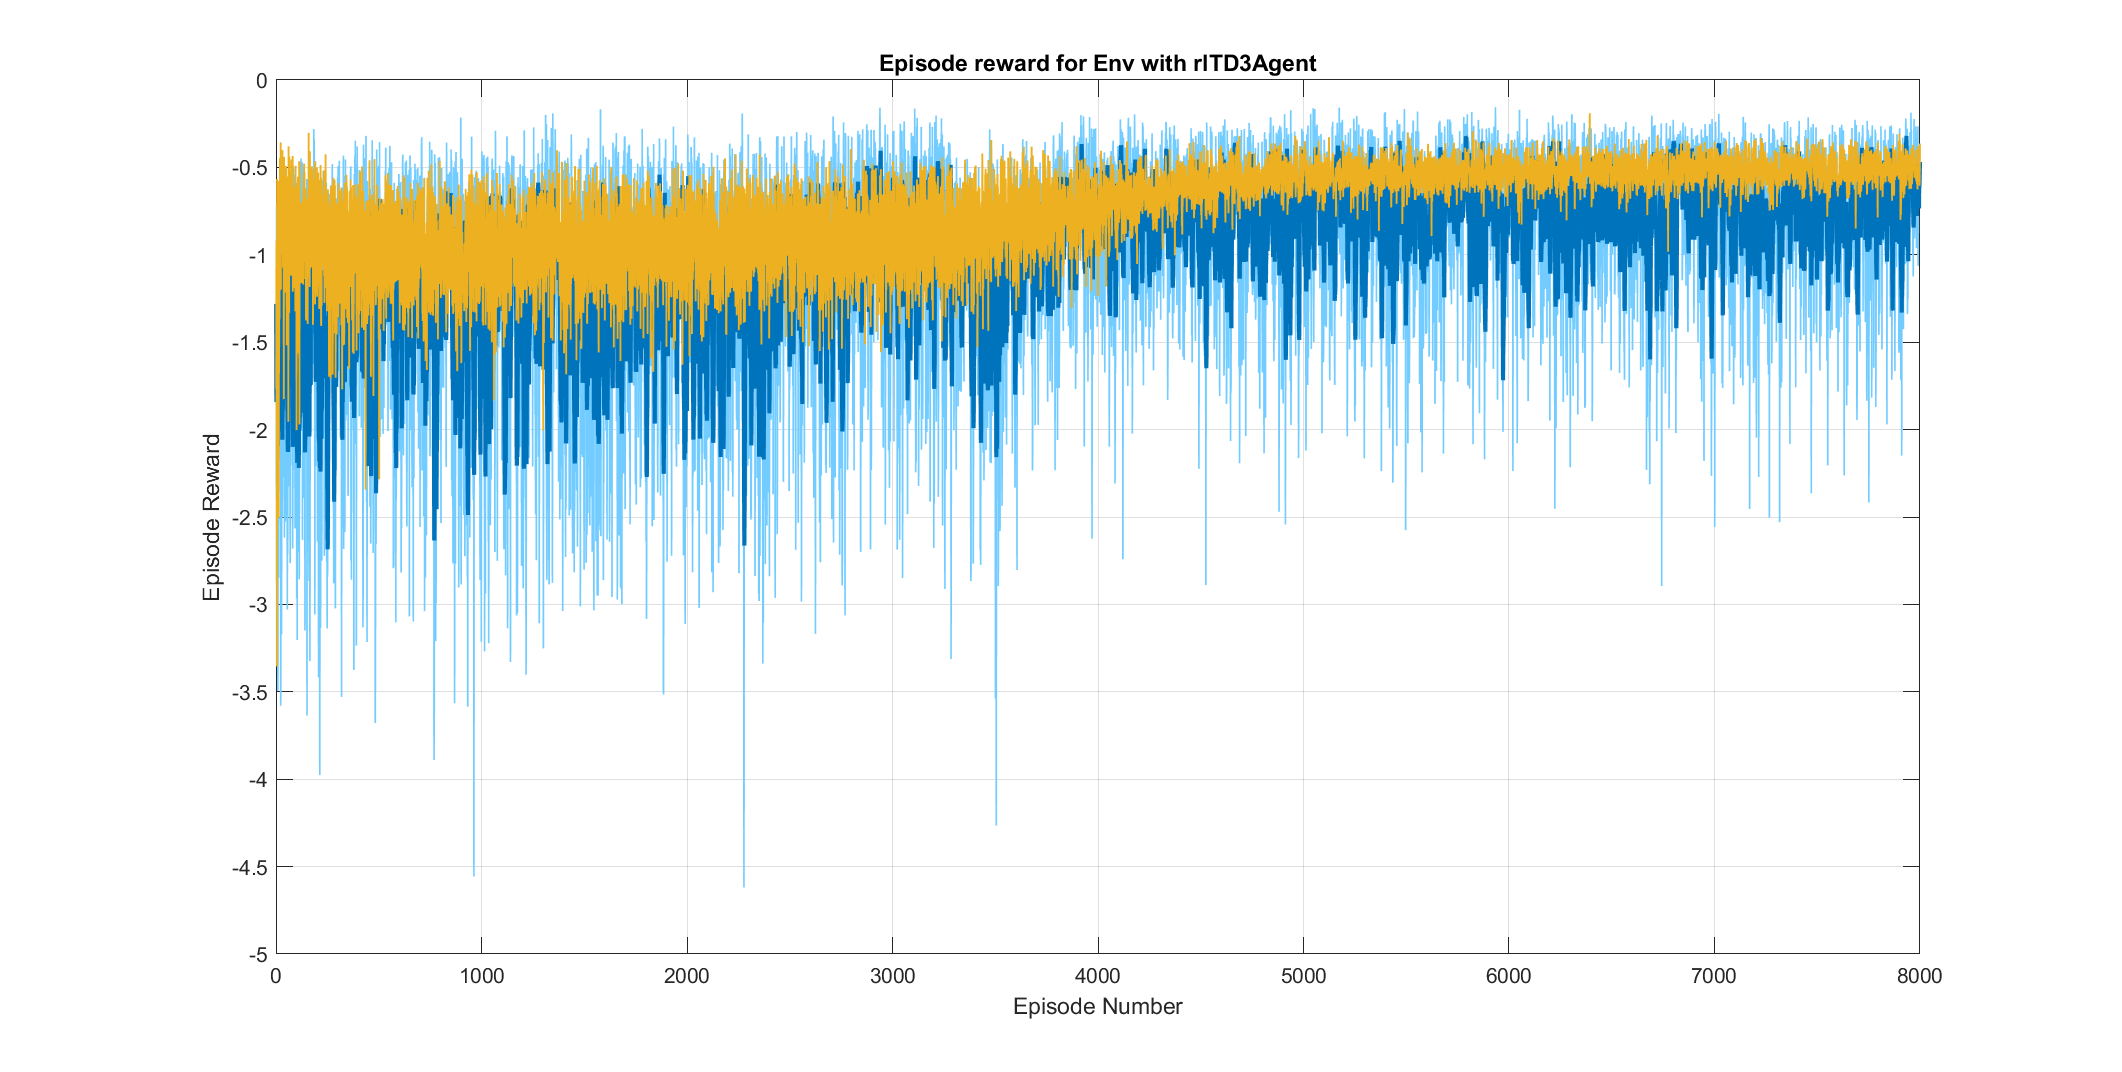
\includegraphics[width=\linewidth,height=0.34\textheight,keepaspectratio]{figures/training_progress_8000eps_valid_baseline.png}

\vspace{0.03cm}
\tiny\textbf{Test visual del benchmark}\par
\vspace{0.01cm}
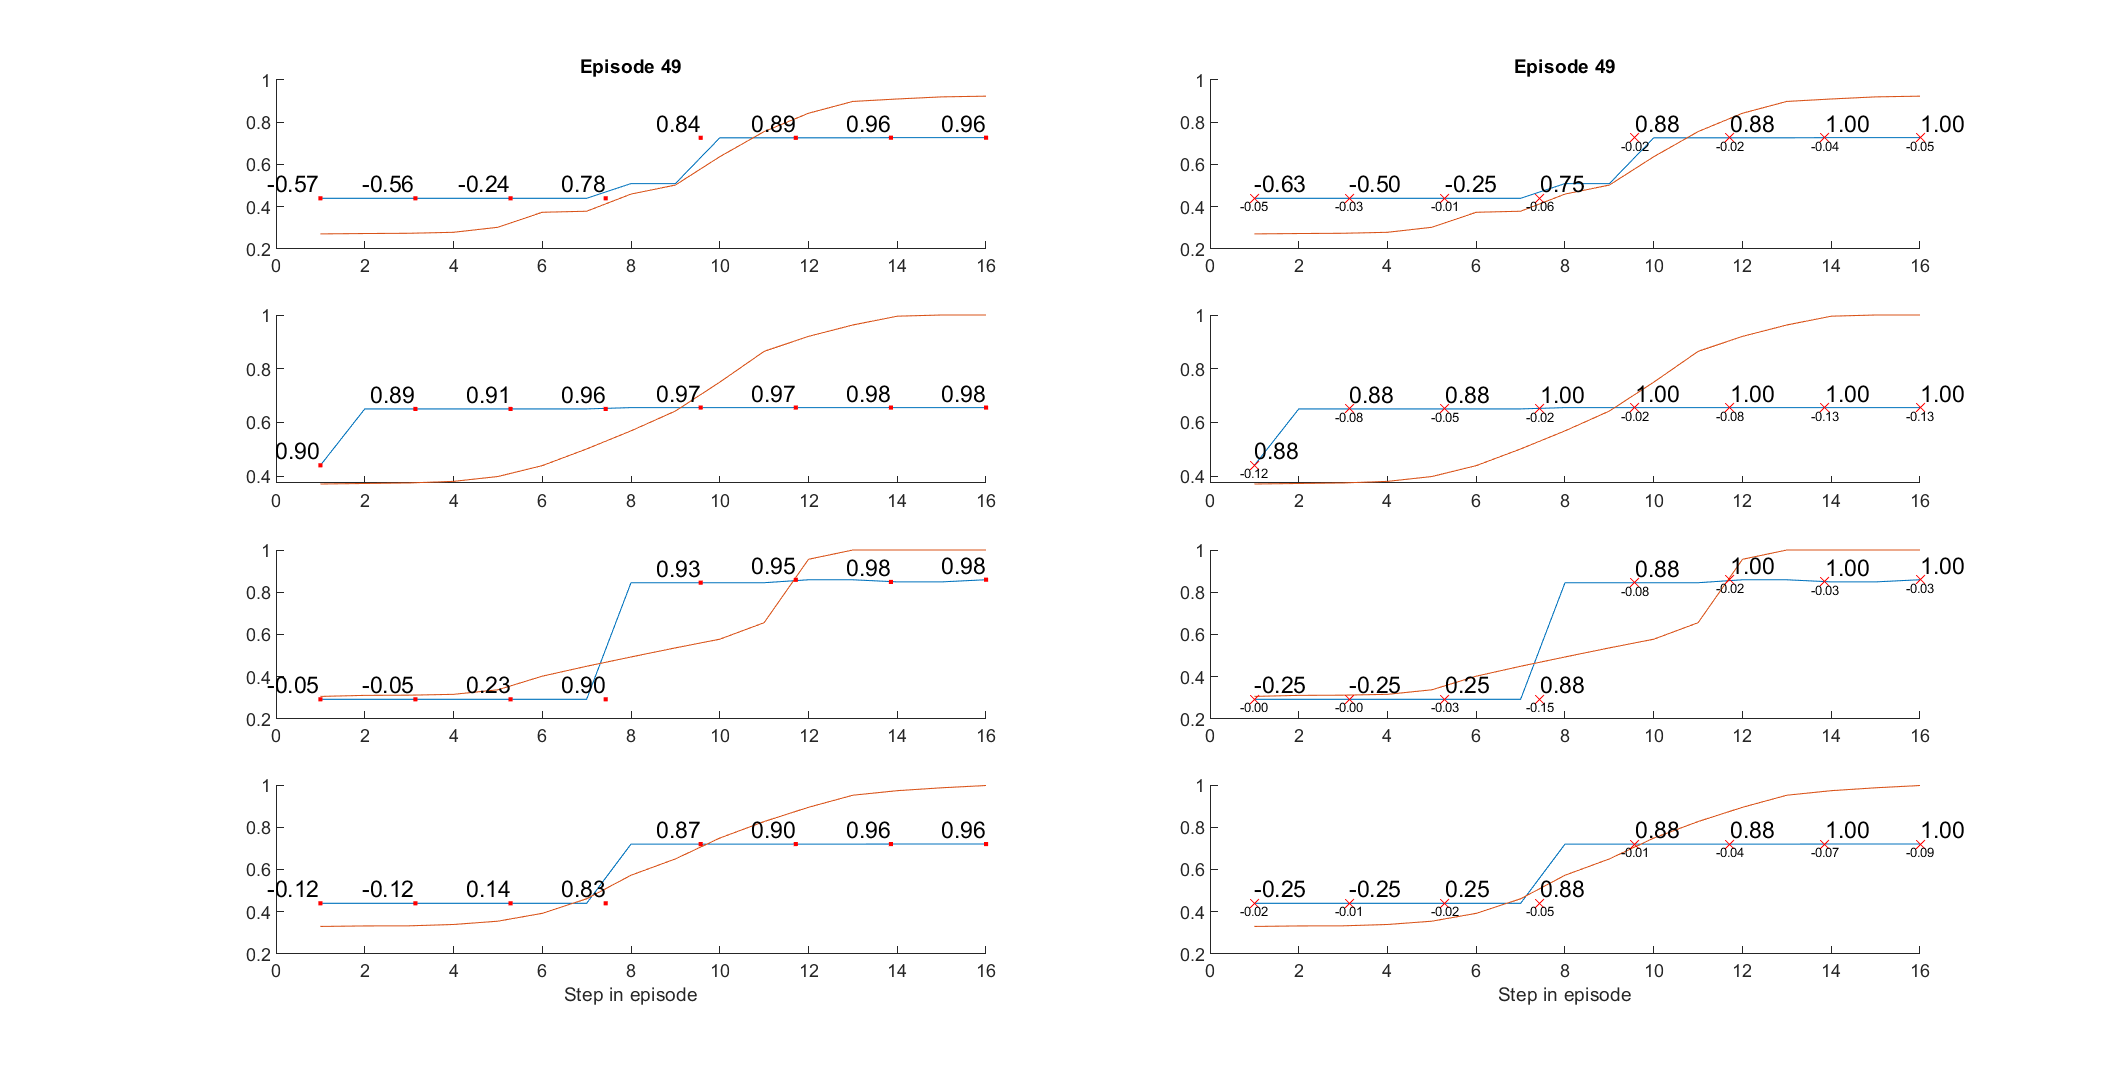
\includegraphics[width=\linewidth,height=0.34\textheight,keepaspectratio]{figures/test_episode_49_valid_baseline_8000.png}
\end{column}
\end{columns}
\end{frame}

\begin{frame}{Por que no bastaba con \texttt{Agent7250}}
\begin{columns}[T]
\begin{column}{0.56\linewidth}
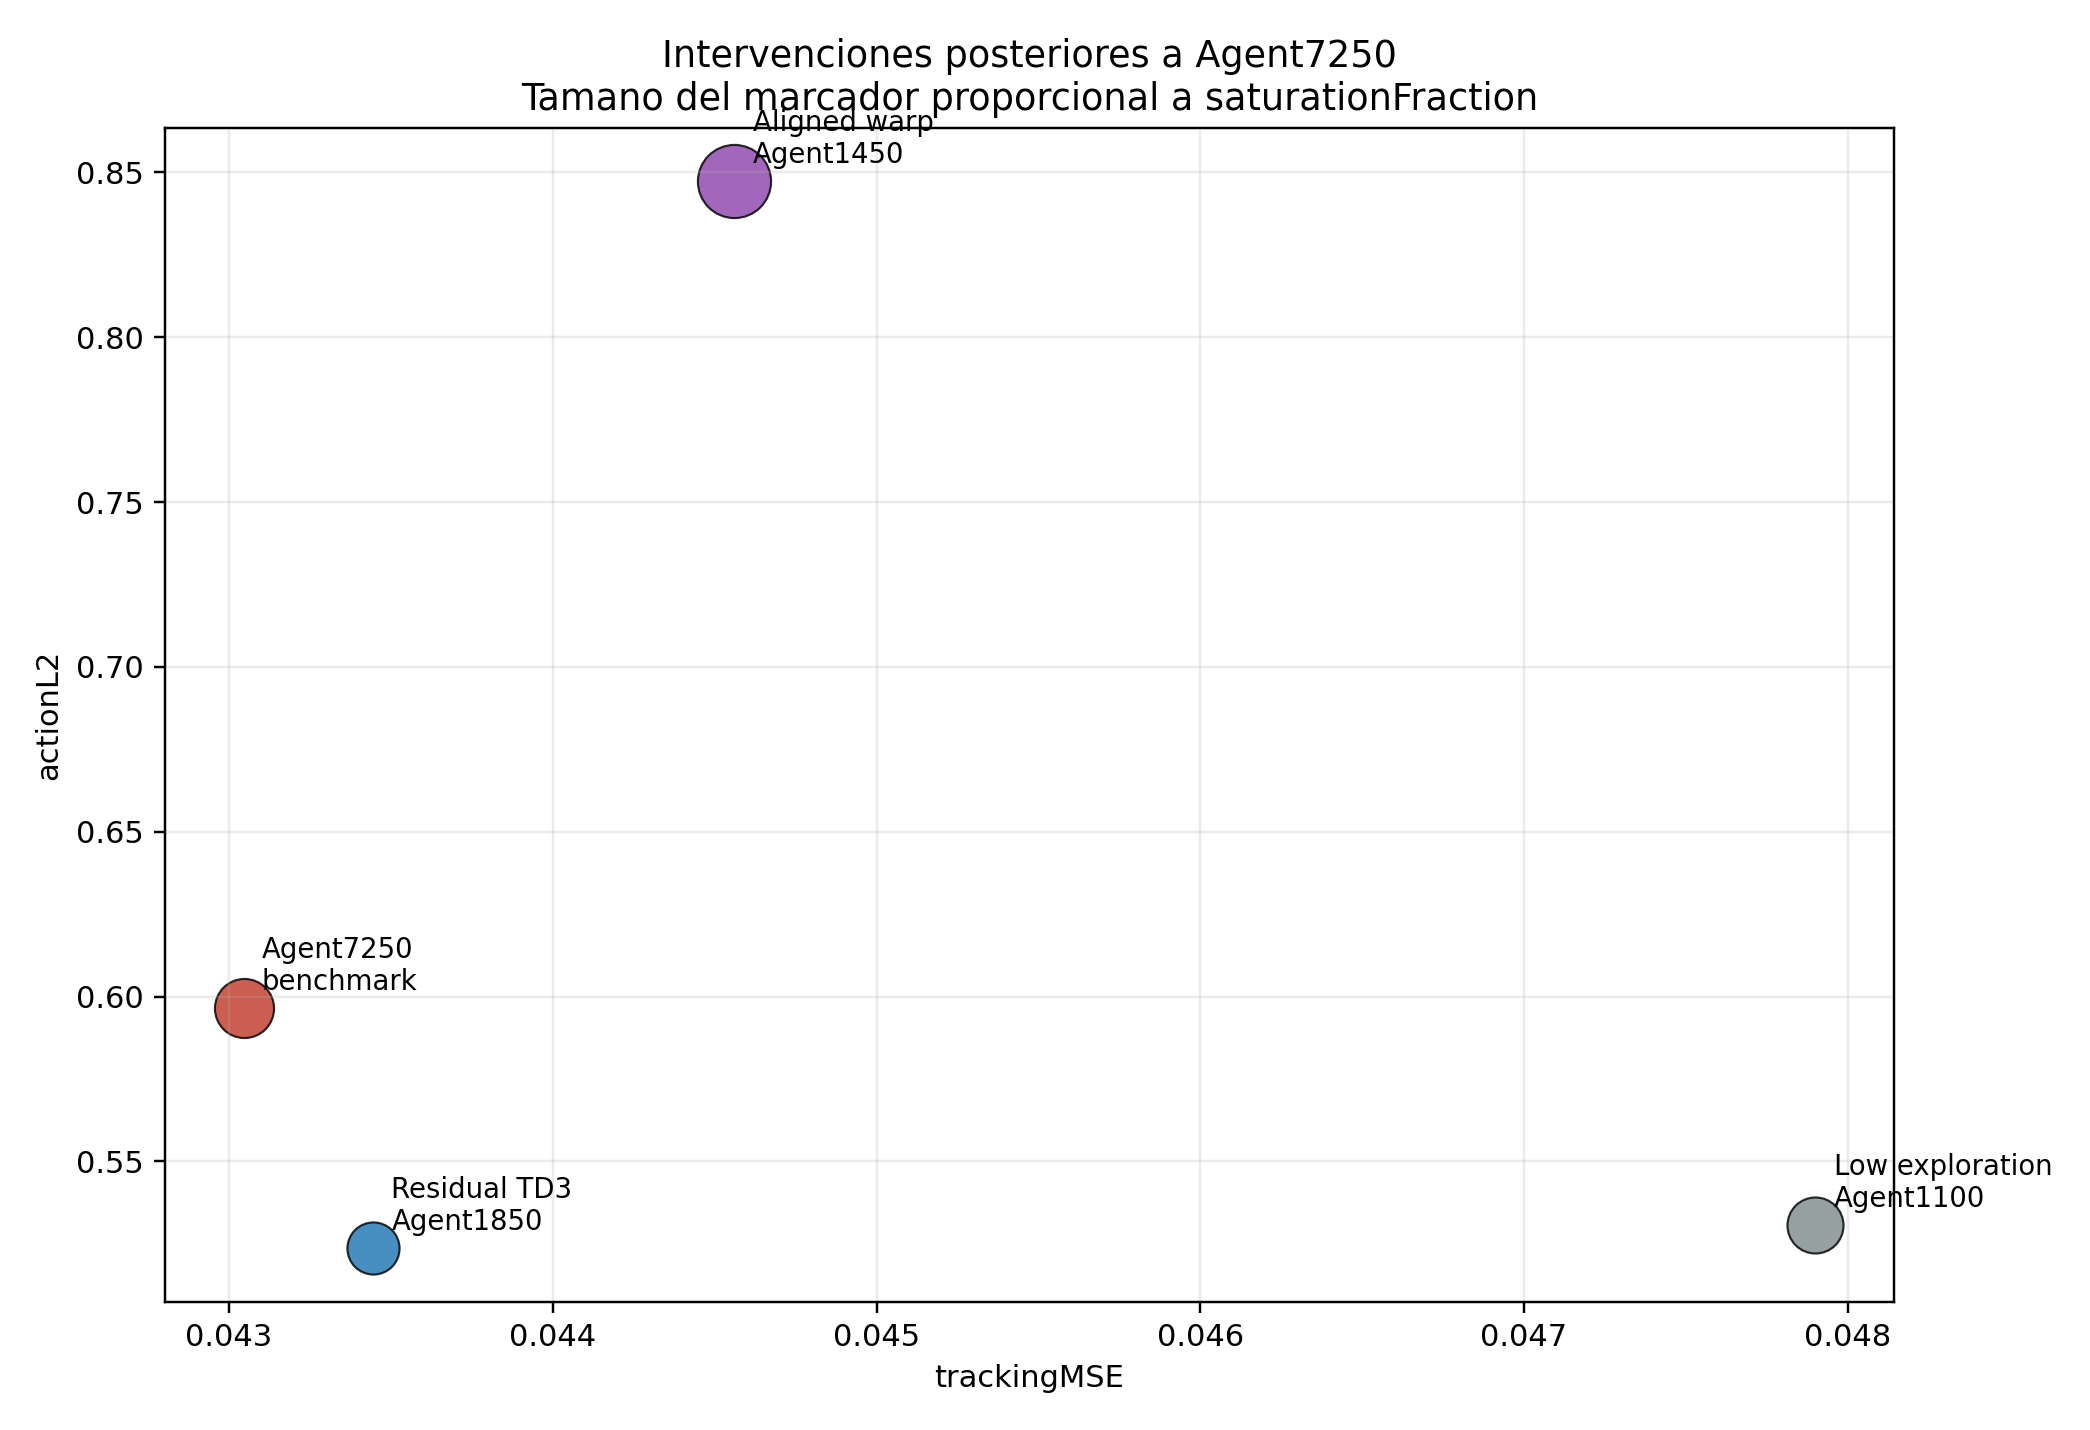
\includegraphics[width=\linewidth]{figures/post7250_interventions_tradeoff_20260326.png}
\end{column}
\begin{column}{0.40\linewidth}
\begin{block}{Nueva pregunta}
\begin{itemize}
\item mantener el tracking
\item bajar saturacion
\item bajar esfuerzo
\item bajar agresividad
\end{itemize}
\end{block}

\begin{alertblock}{Problema observado}
Las primeras ideas post-\texttt{7250} se fueron a dos extremos:
\begin{itemize}
\item demasiado timidas
\item demasiado agresivas
\end{itemize}
\end{alertblock}
\end{column}
\end{columns}
\end{frame}

\begin{frame}{Experimentos post-\texttt{7250} en una sola vista}
\small
\begin{tabularx}{\linewidth}{@{}p{3.5cm}X X@{}}
\toprule
Idea & Por que parecia buena & Resultado \\
\midrule
Baja exploracion & Suavizar una politica ya buena & Mejoro suavidad, pero perdio tracking. \\
Reward de saturacion & Castigar el borde del actuador & Politica demasiado timida. \\
Warm-start offline & Meter un prior suave & Demasiado conservador. \\
Warp alineada al actuador & Reducir hueco entre accion y PWM & Politica demasiado agresiva. \\
Residual TD3 & Corregir la politica buena sin reemplazarla & \textbf{Primera mejora aceptable}. \\
\bottomrule
\end{tabularx}

\vspace{0.4cm}
\small
La leccion fue clara: no convenia rehacer toda la politica; convenia corregir una politica ya fuerte.
\end{frame}

\begin{frame}{Idea clave: politica residual}
\begin{columns}[T]
\begin{column}{0.56\linewidth}
\[
a_{\mathrm{final}} = \mathrm{clip}\left(a_{\mathrm{base}} + \alpha_{\mathrm{res}}\, a_{\mathrm{corr}}, -1, 1\right)
\]

\begin{block}{Interpretacion}
\begin{itemize}
\item \(a_{\mathrm{base}}\): accion de \texttt{Agent7250}
\item \(a_{\mathrm{corr}}\): correccion aprendida
\item \(\alpha_{\mathrm{res}}\): cuanto dejamos corregir
\end{itemize}
\end{block}
\end{column}
\begin{column}{0.40\linewidth}
\begin{block}{Por que tenia sentido}
\begin{itemize}
\item \texttt{Agent7250} ya hacia buen tracking
\item mover toda la politica era riesgoso
\item una correccion pequena es mas estable
\end{itemize}
\end{block}

\begin{alertblock}{Lectura del alpha}
\begin{itemize}
\item muy bajo: corrige poco
\item muy alto: rompe el equilibrio
\item intermedio: mejor compromiso
\end{itemize}
\end{alertblock}
\end{column}
\end{columns}

\vspace{0.2cm}
\tiny Fuentes clave: Residual Policy Learning (Silver et al., 2018), Schaff and Walter (2020), ResFiT (2025).
\end{frame}

\begin{frame}{Configuracion de la fase residual}
\begin{columns}[T]
\begin{column}{0.48\linewidth}
\begin{block}{Se mantuvo fijo}
\begin{itemize}
\item \texttt{markov52}
\item TD3 feedforward
\item \texttt{trackingMseActionRateReward}
\item cuantizacion del actuador
\item politica base = \texttt{Agent7250}
\end{itemize}
\end{block}
\end{column}
\begin{column}{0.48\linewidth}
\begin{block}{Se ajusto}
\begin{itemize}
\item \(\alpha_{\mathrm{res}}\)
\item exploracion residual baja
\item auditoria por checkpoints
\item test visual de 50 simulaciones
\end{itemize}
\end{block}

\begin{block}{Valor final}
\[
\alpha_{\mathrm{res}} = 0.20
\]
\end{block}
\end{column}
\end{columns}
\end{frame}

\begin{frame}{Grafica de aprendizaje}
\begin{columns}[T]
\begin{column}{0.56\linewidth}
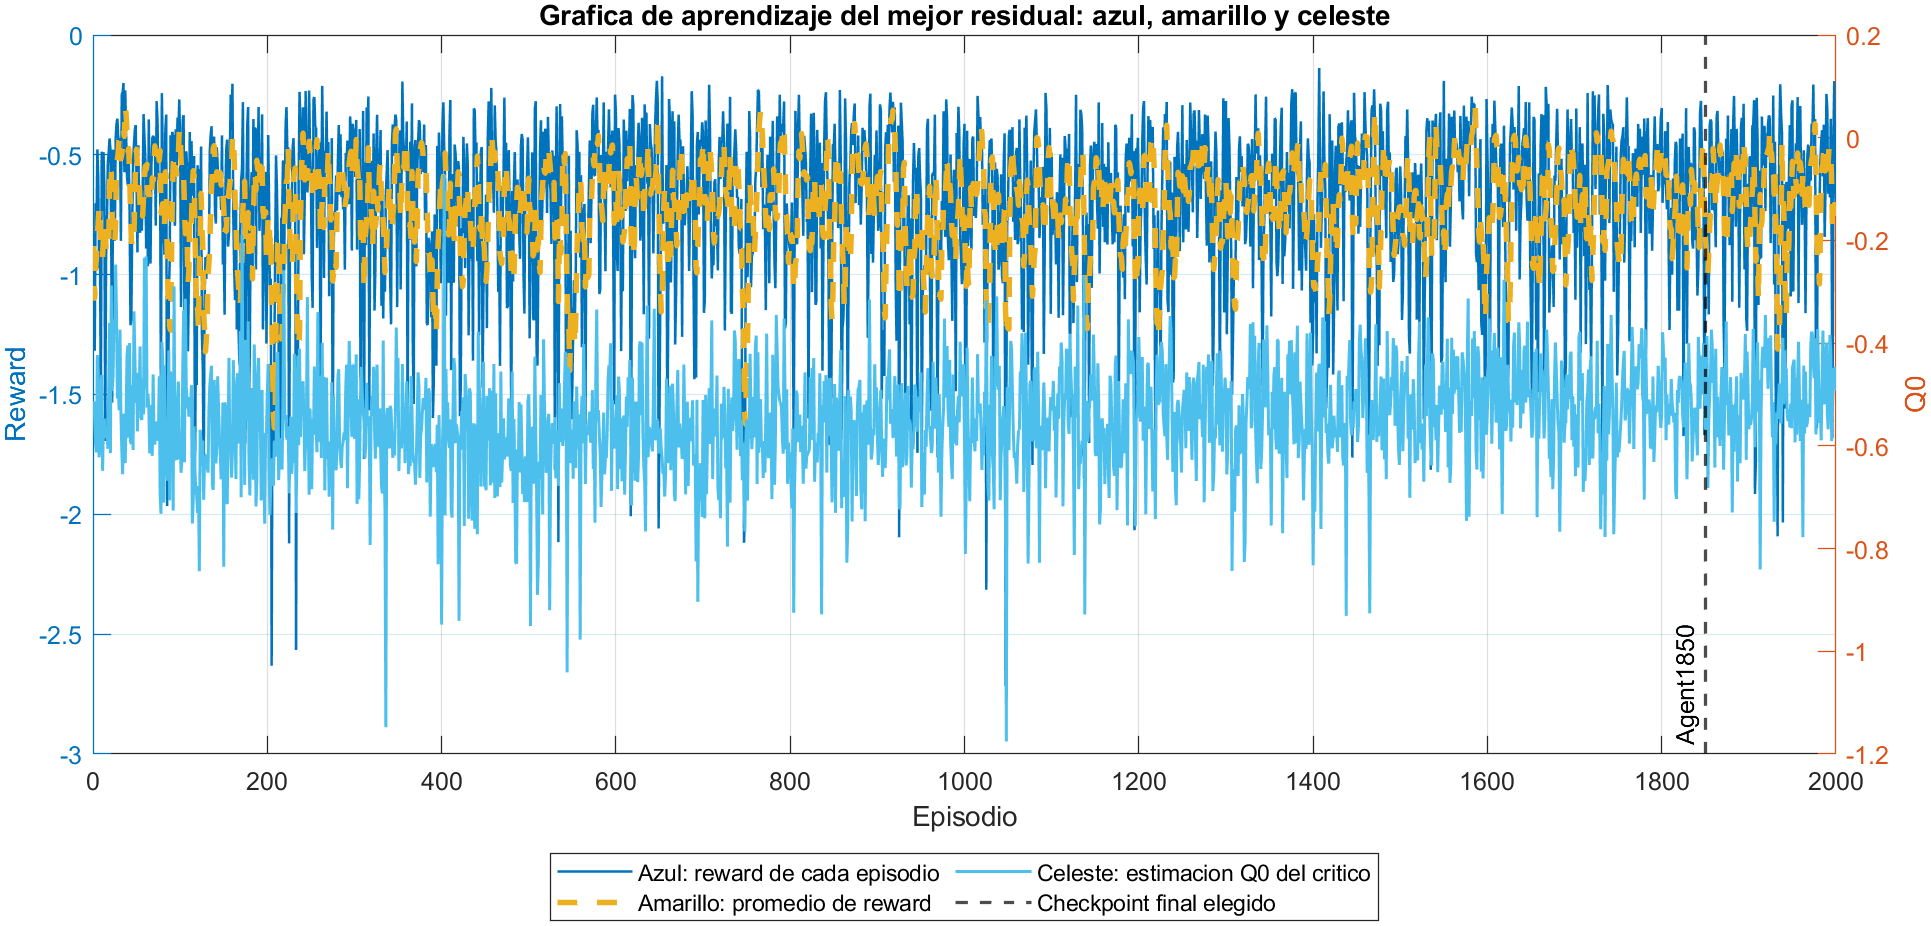
\includegraphics[width=\linewidth]{figures/charla_training_residual_20260326.png}
\end{column}
\begin{column}{0.38\linewidth}
\footnotesize
\begin{block}{Azul}
Reward de cada episodio. Puede oscilar bastante.
\end{block}
\begin{block}{Amarillo}
Promedio de reward. Sirve para ver la tendencia real.
\end{block}
\begin{block}{Celeste}
\texttt{Q0}. Es una estimacion interna del valor esperado.
\end{block}
\begin{alertblock}{Linea negra}
Marca \texttt{Agent1850}, el checkpoint elegido por auditoria y test.
\end{alertblock}
\end{column}
\end{columns}
\end{frame}

\begin{frame}{Como leer el test del residual}
\begin{columns}[T]
\begin{column}{0.62\linewidth}
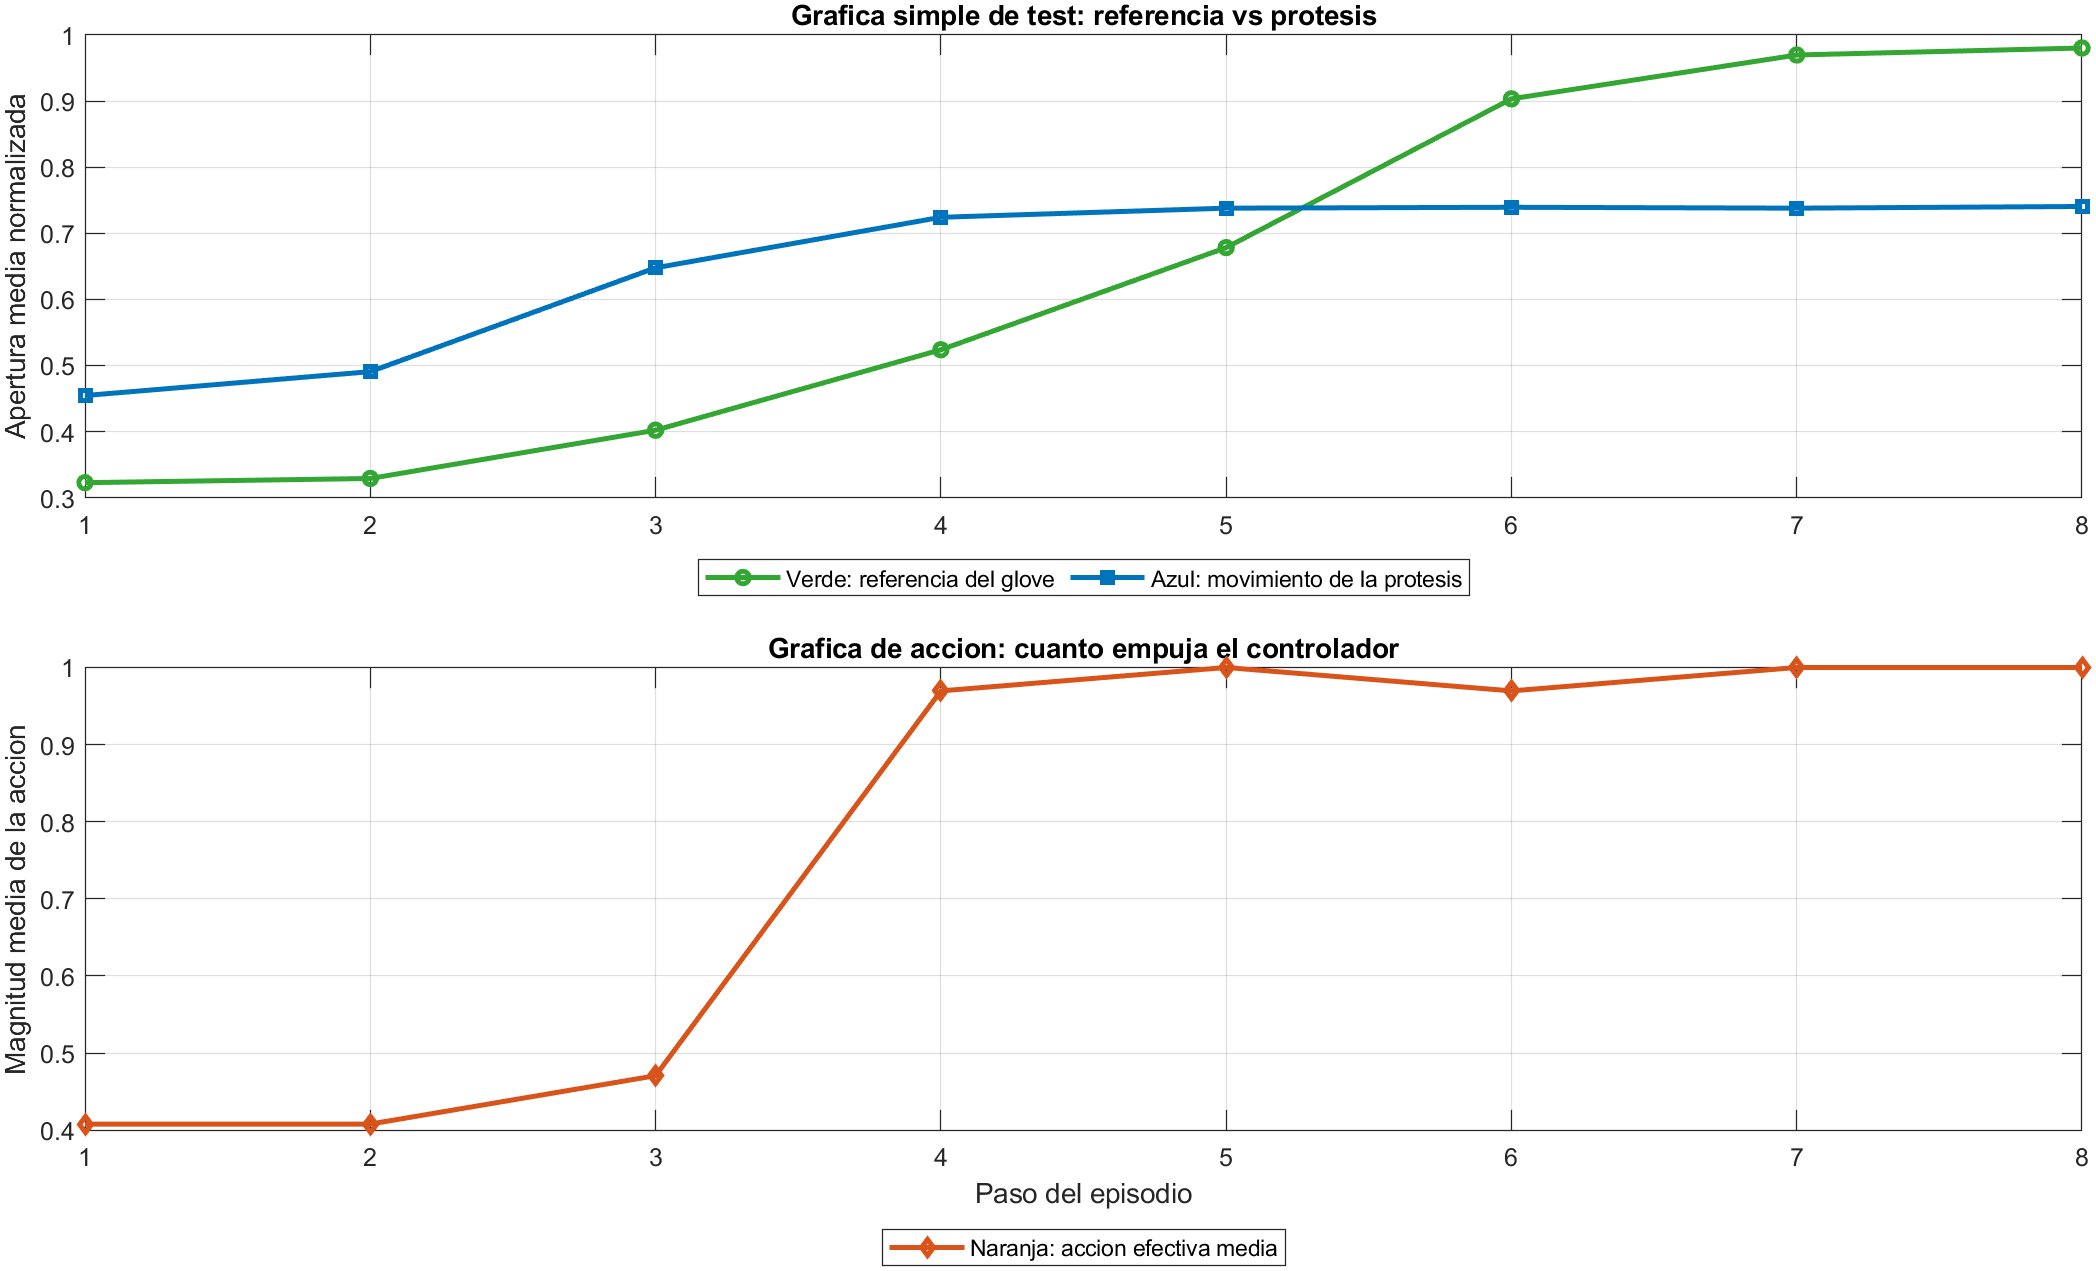
\includegraphics[width=\linewidth]{figures/charla_test_residual_20260326.png}
\end{column}
\begin{column}{0.34\linewidth}
\begin{block}{Verde}
Referencia del glove.
\end{block}
\begin{block}{Azul}
Movimiento real de la protesis.
\end{block}
\begin{block}{Naranja}
Magnitud media de la accion.
\end{block}

\small
Si azul sigue a verde, hay buen tracking.\\
Si naranja no se dispara, la politica no esta empujando de mas.
\end{column}
\end{columns}
\end{frame}

\begin{frame}{Barridos de alpha}
\begin{columns}[T]
\begin{column}{0.58\linewidth}
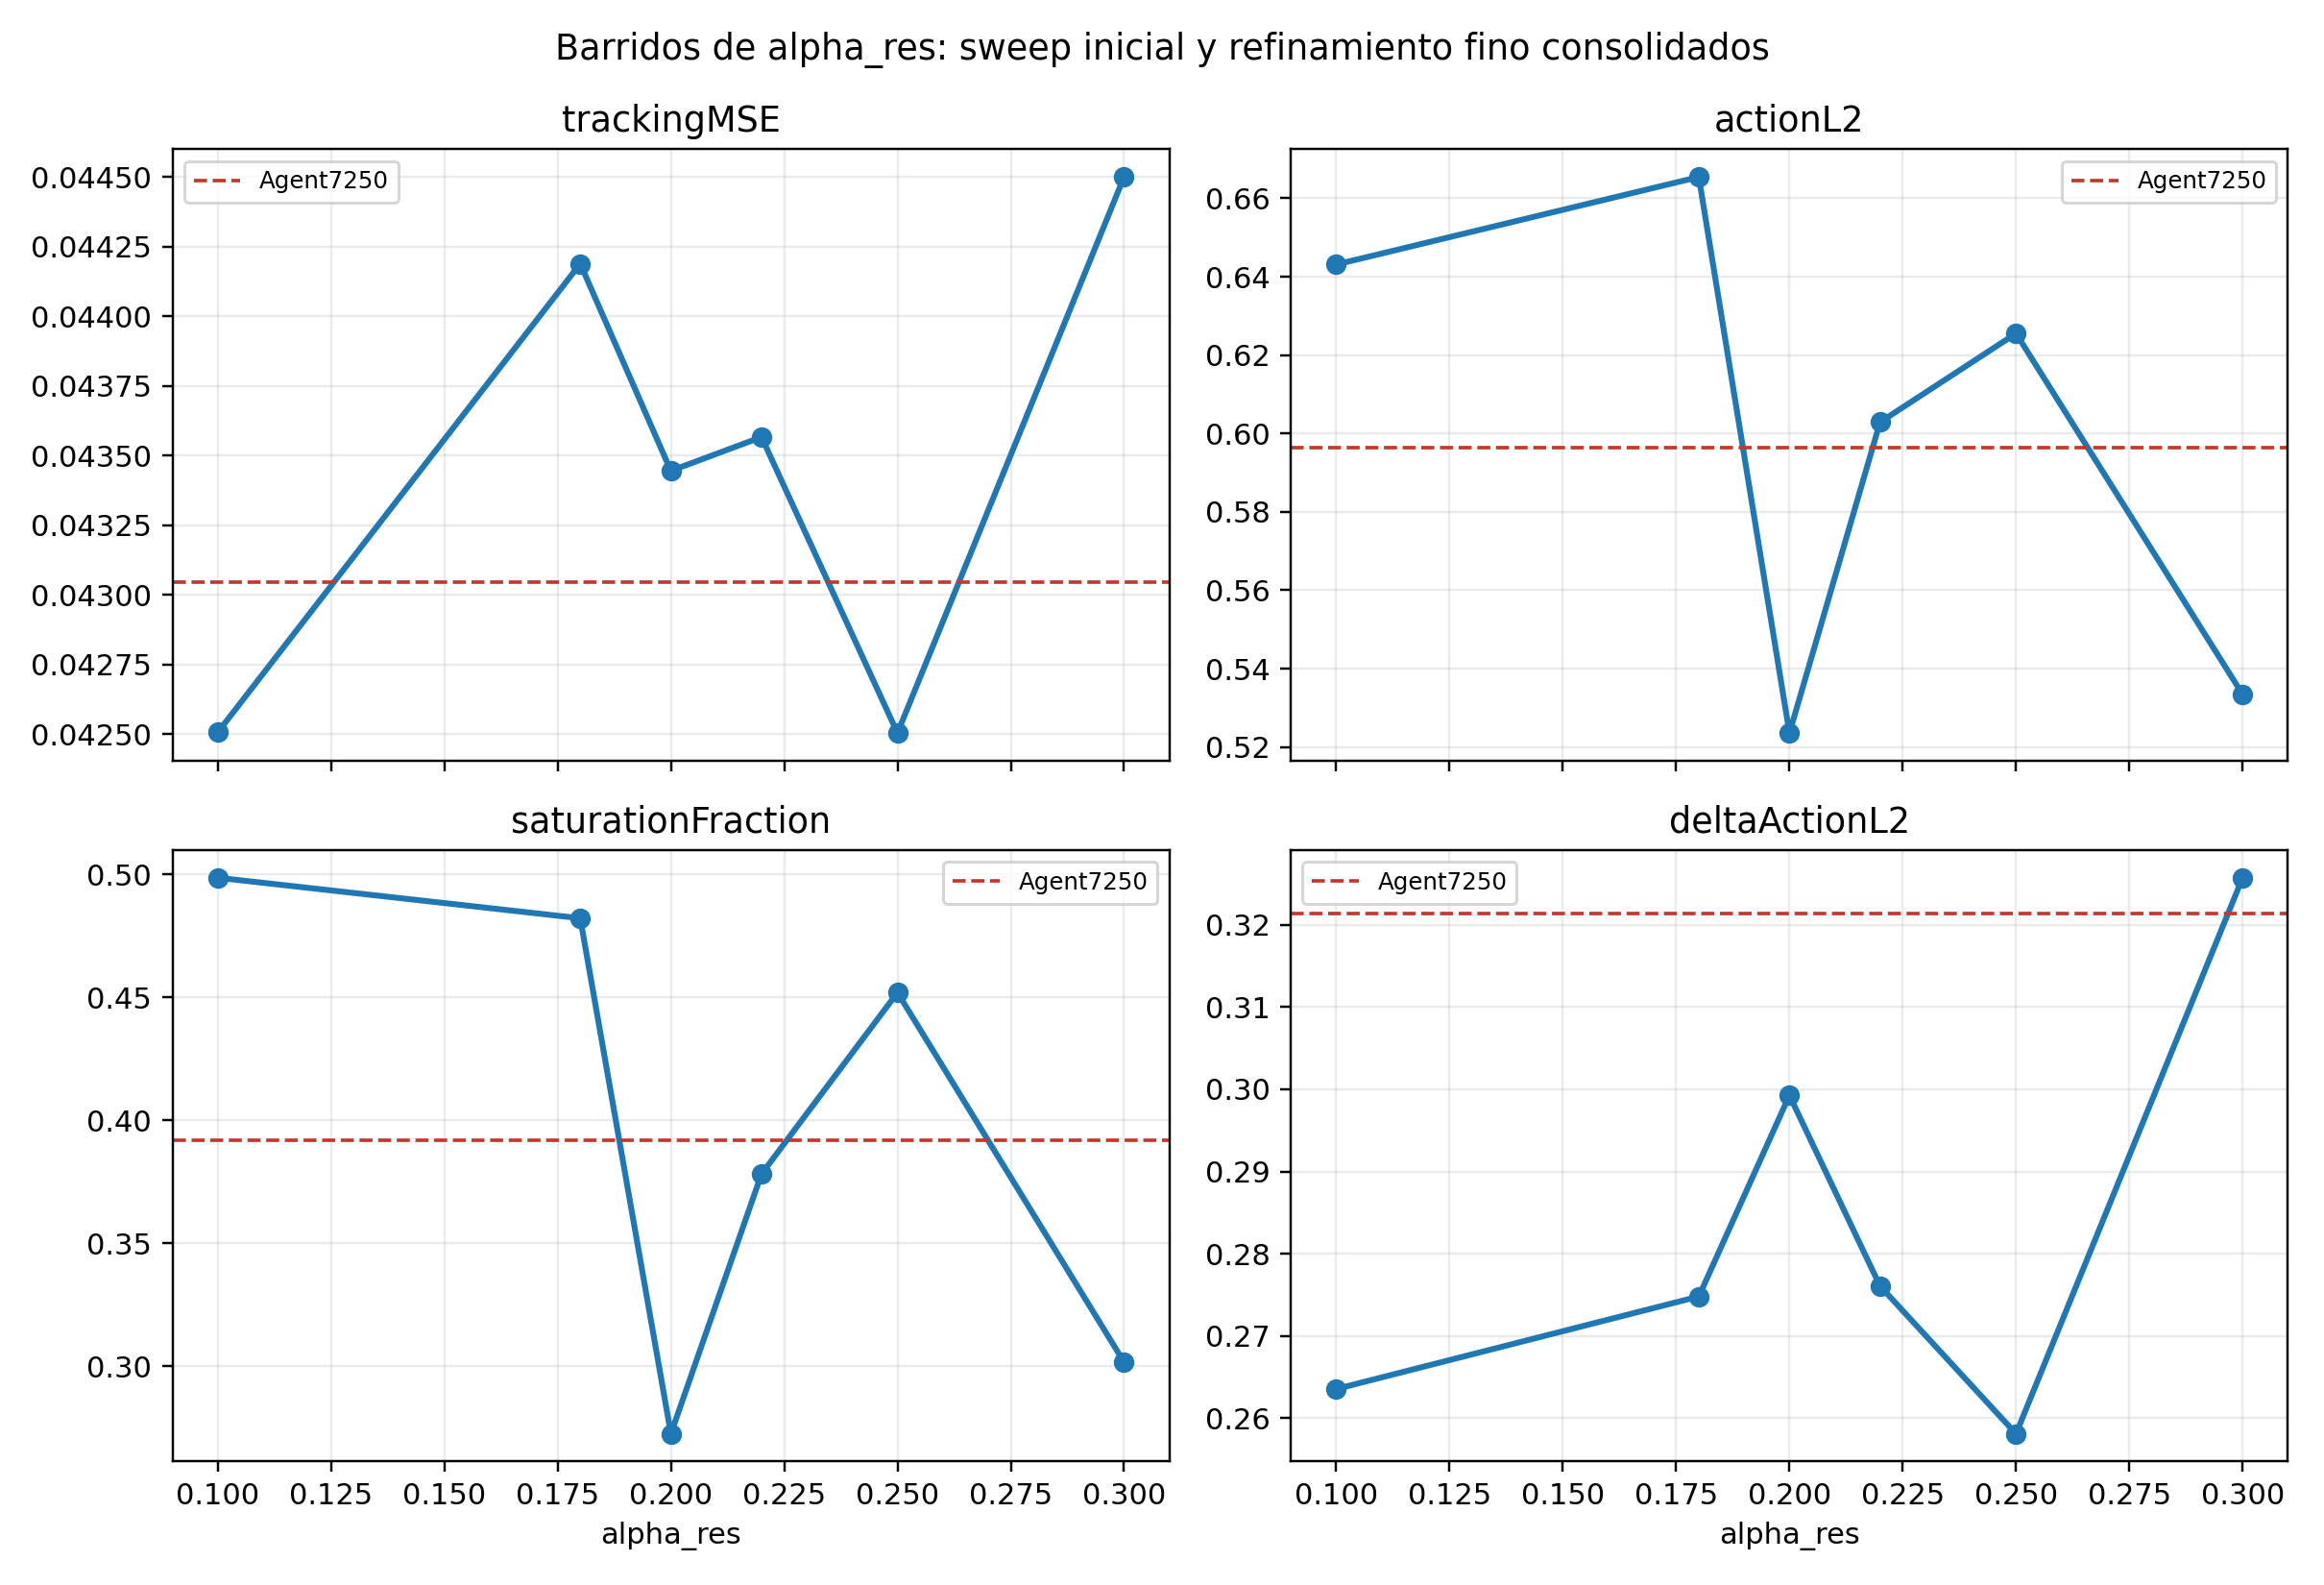
\includegraphics[width=\linewidth]{figures/residual_alpha_sweep_metrics_20260326.png}
\end{column}
\begin{column}{0.38\linewidth}
\begin{block}{Barrido corto}
\[
0.10,\; 0.20,\; 0.30
\]
\end{block}
\begin{block}{Refinamiento fino}
\[
0.18,\; 0.20,\; 0.22,\; 0.25
\]
\end{block}
\begin{alertblock}{Conclusion}
\(\alpha = 0.20\) fue el mejor punto intermedio.\\
El refinamiento fino lo confirmo.
\end{alertblock}
\end{column}
\end{columns}
\end{frame}

\begin{frame}{Comparacion del articulo base al resultado final}
\small
\begin{columns}[T]
\begin{column}{0.63\linewidth}
\setlength{\tabcolsep}{3pt}
\centering
\resizebox{\linewidth}{!}{%
\begin{tabular}{lcccc}
\toprule
Metrica & Articulo base & Post-fix 2000 & \texttt{Agent7250} & Residual \texttt{Agent1850} \\
\midrule
trackingMSE & -- & 0.052805 & 0.043045 & 0.043445 \\
trackingMAE & 0.1553* & 0.179093 & 0.160336 & 0.163542 \\
actionL2 & -- & 0.674957 & 0.596444 & 0.523597 \\
saturationFraction & -- & 0.474999 & 0.392086 & 0.272637 \\
deltaActionL2 & -- & 0.633264 & 0.321385 & 0.299262 \\
\bottomrule
\end{tabular}
}

\vspace{0.15cm}
\begin{block}{Comparacion}
\scriptsize
* El articulo base reporta MAE medio de simulacion y un error aproximado del 10 al 15 por ciento. No reporta \texttt{actionL2}, \texttt{saturationFraction} ni \texttt{deltaActionL2}, asi que funciona como referencia historica y no como comparacion completa.
\end{block}
\end{column}
\begin{column}{0.30\linewidth}
\centering
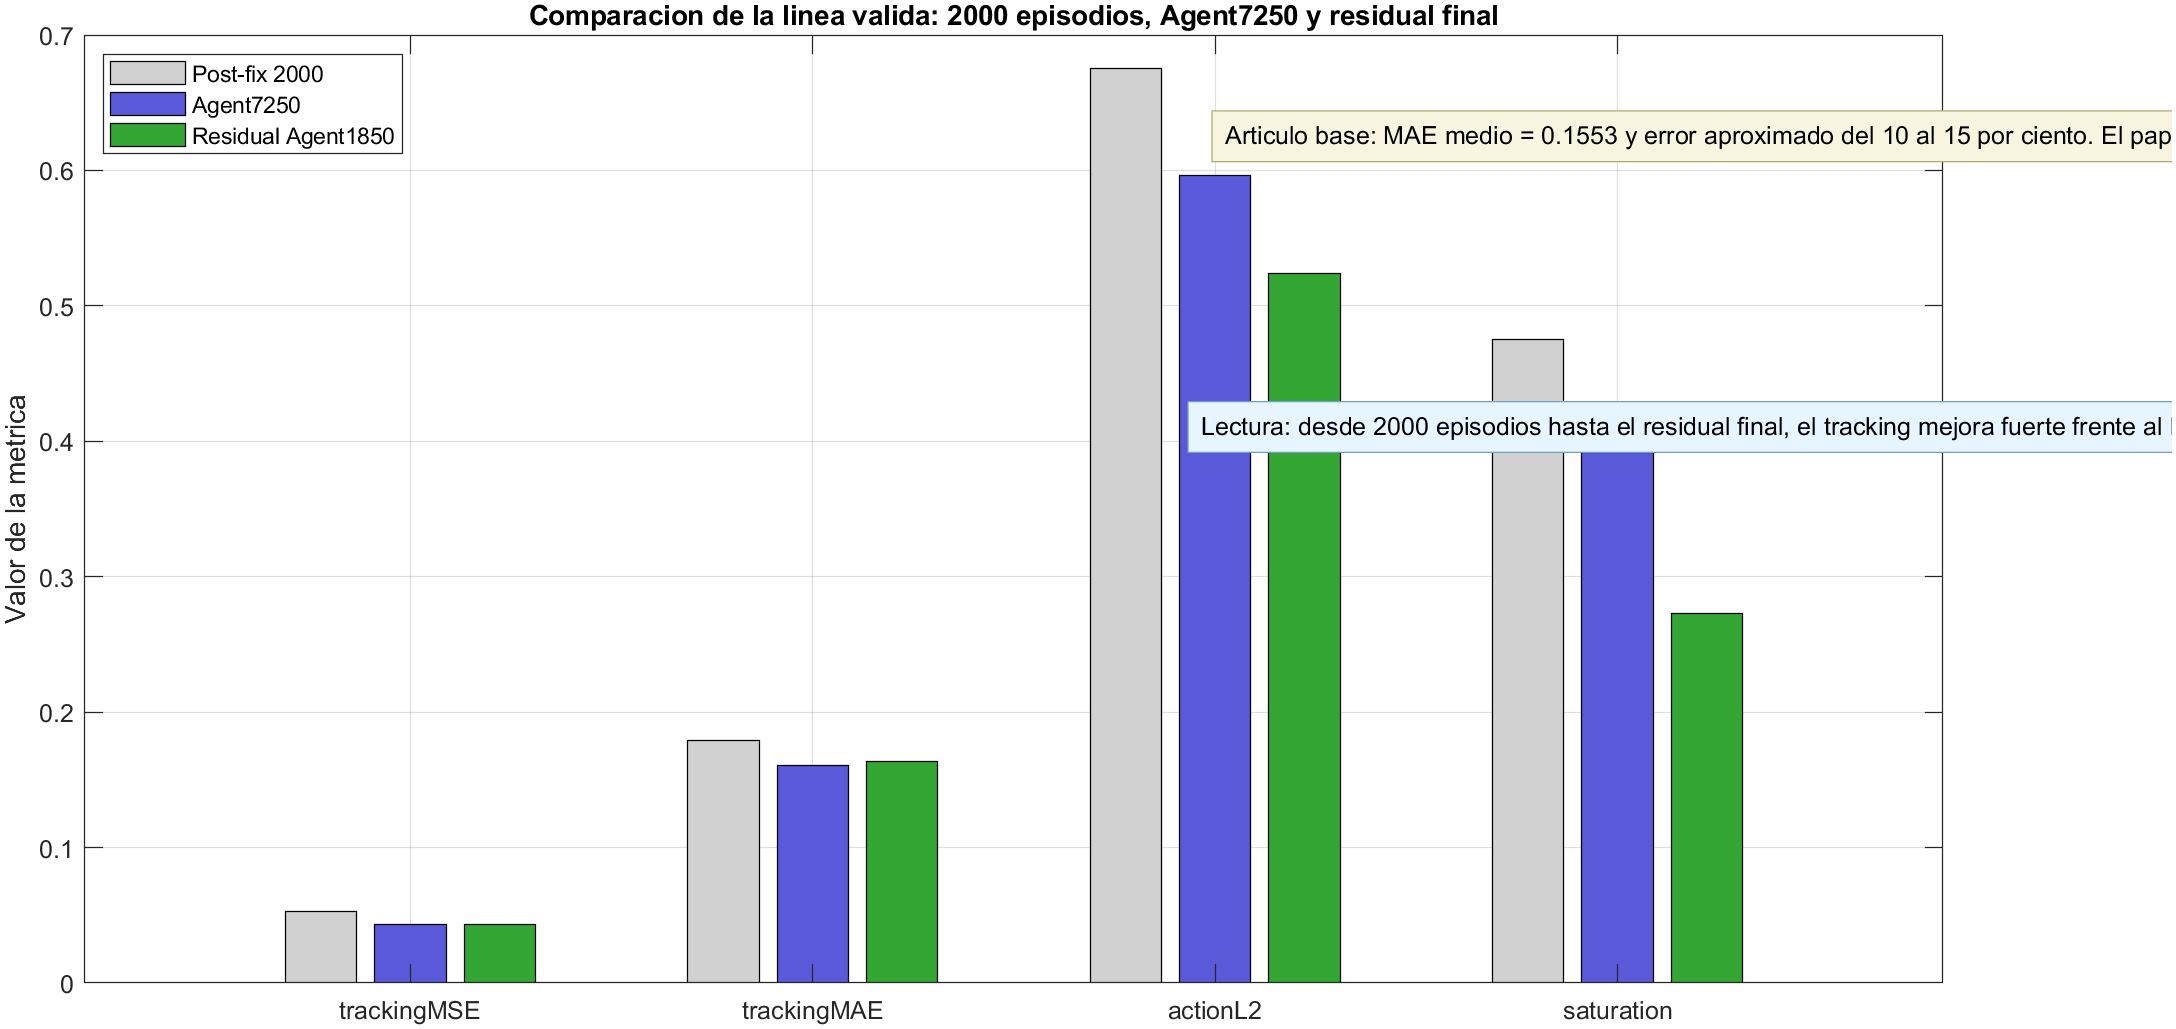
\includegraphics[width=0.82\linewidth]{figures/charla_comparacion_base_a_final_20260326.png}

\vspace{0.18cm}
\begin{exampleblock}{Lectura del resultado}
\scriptsize
El residual final mantiene casi el tracking de \texttt{Agent7250}, pero reduce esfuerzo y saturacion con una mejora clara.
\end{exampleblock}
\end{column}
\end{columns}
\end{frame}

\begin{frame}{Lectura final del resultado}
\begin{columns}[T]
\begin{column}{0.48\linewidth}
\begin{block}{Que gano el residual}
\begin{itemize}
\item baja esfuerzo total
\item baja saturacion
\item baja brusquedad
\item conserva casi el tracking
\end{itemize}
\end{block}
\end{column}
\begin{column}{0.48\linewidth}
\begin{alertblock}{Que no hizo}
No gano por tracking puro.\\
La mejora fue de \textbf{compromiso}, no de un solo numero.
\end{alertblock}

\begin{block}{Decision final}
\texttt{Agent1850} se toma como punto final operativo porque cumple \texttt{ConditionB}.
\end{block}
\end{column}
\end{columns}
\end{frame}

\begin{frame}{Fuentes clave}
\small
\begin{itemize}
\item Fuertes Bustos et al., \emph{Continuous Operation of a Myoelectric Hand Prosthesis using the TD3 Reinforcement Learning Algorithm}.
\item Fujimoto, van Hoof y Meger (2018), \emph{Addressing Function Approximation Error in Actor-Critic Methods}.
\item Chen et al. (2023), \emph{A Review of Myoelectric Control for Prosthetic Hand Manipulation}.
\item Silver et al. (2018), \emph{Residual Policy Learning}.
\item Schaff y Walter (2020), \emph{Residual Policy Learning for Shared Autonomy}.
\item MathWorks, documentacion de \texttt{rlTD3Agent}, \texttt{rlTD3AgentOptions} y \texttt{rlContinuousDeterministicActor}.
\end{itemize}

\vfill
\centering
\Large Preguntas
\end{frame}

\end{document}
